\documentclass[1p]{elsarticle_modified}
%\bibliographystyle{elsarticle-num}

%\usepackage[colorlinks]{hyperref}
%\usepackage{abbrmath_seonhwa} %\Abb, \Ascr, \Acal ,\Abf, \Afrak
\usepackage{amsfonts}
\usepackage{amssymb}
\usepackage{amsmath}
\usepackage{amsthm}
\usepackage{scalefnt}
\usepackage{amsbsy}
\usepackage{kotex}
\usepackage{caption}
\usepackage{subfig}
\usepackage{color}
\usepackage{graphicx}
\usepackage{xcolor} %% white, black, red, green, blue, cyan, magenta, yellow
\usepackage{float}
\usepackage{setspace}
\usepackage{hyperref}

\usepackage{tikz}
\usetikzlibrary{arrows}

\usepackage{multirow}
\usepackage{array} % fixed length table
\usepackage{hhline}

%%%%%%%%%%%%%%%%%%%%%
\makeatletter
\renewcommand*\env@matrix[1][\arraystretch]{%
	\edef\arraystretch{#1}%
	\hskip -\arraycolsep
	\let\@ifnextchar\new@ifnextchar
	\array{*\c@MaxMatrixCols c}}
\makeatother %https://tex.stackexchange.com/questions/14071/how-can-i-increase-the-line-spacing-in-a-matrix
%%%%%%%%%%%%%%%

\usepackage[normalem]{ulem}

\newcommand{\msout}[1]{\ifmmode\text{\sout{\ensuremath{#1}}}\else\sout{#1}\fi}
%SOURCE: \msout is \stkout macro in https://tex.stackexchange.com/questions/20609/strikeout-in-math-mode

\newcommand{\cancel}[1]{
	\ifmmode
	{\color{red}\msout{#1}}
	\else
	{\color{red}\sout{#1}}
	\fi
}

\newcommand{\add}[1]{
	{\color{blue}\uwave{#1}}
}

\newcommand{\replace}[2]{
	\ifmmode
	{\color{red}\msout{#1}}{\color{blue}\uwave{#2}}
	\else
	{\color{red}\sout{#1}}{\color{blue}\uwave{#2}}
	\fi
}

\newcommand{\Sol}{\mathcal{S}} %segment
\newcommand{\D}{D} %diagram
\newcommand{\A}{\mathcal{A}} %arc


%%%%%%%%%%%%%%%%%%%%%%%%%%%%%5 test

\def\sl{\operatorname{\textup{SL}}(2,\Cbb)}
\def\psl{\operatorname{\textup{PSL}}(2,\Cbb)}
\def\quan{\mkern 1mu \triangleright \mkern 1mu}

\theoremstyle{definition}
\newtheorem{thm}{Theorem}[section]
\newtheorem{prop}[thm]{Proposition}
\newtheorem{lem}[thm]{Lemma}
\newtheorem{ques}[thm]{Question}
\newtheorem{cor}[thm]{Corollary}
\newtheorem{defn}[thm]{Definition}
\newtheorem{exam}[thm]{Example}
\newtheorem{rmk}[thm]{Remark}
\newtheorem{alg}[thm]{Algorithm}

\newcommand{\I}{\sqrt{-1}}
\begin{document}

%\begin{frontmatter}
%
%\title{Boundary parabolic representations of knots up to 8 crossings}
%
%%% Group authors per affiliation:
%\author{Yunhi Cho} 
%\address{Department of Mathematics, University of Seoul, Seoul, Korea}
%\ead{yhcho@uos.ac.kr}
%
%
%\author{Seonhwa Kim} %\fnref{s_kim}}
%\address{Center for Geometry and Physics, Institute for Basic Science, Pohang, 37673, Korea}
%\ead{ryeona17@ibs.re.kr}
%
%\author{Hyuk Kim}
%\address{Department of Mathematical Sciences, Seoul National University, Seoul 08826, Korea}
%\ead{hyukkim@snu.ac.kr}
%
%\author{Seokbeom Yoon}
%\address{Department of Mathematical Sciences, Seoul National University, Seoul, 08826,  Korea}
%\ead{sbyoon15@snu.ac.kr}
%
%\begin{abstract}
%We find all boundary parabolic representation of knots up to 8 crossings.
%
%\end{abstract}
%\begin{keyword}
%    \MSC[2010] 57M25 
%\end{keyword}
%
%\end{frontmatter}

%\linenumbers
%\tableofcontents
%
\newcommand\colored[1]{\textcolor{white}{\rule[-0.35ex]{0.8em}{1.4ex}}\kern-0.8em\color{red} #1}%
%\newcommand\colored[1]{\textcolor{white}{ #1}\kern-2.17ex	\textcolor{white}{ #1}\kern-1.81ex	\textcolor{white}{ #1}\kern-2.15ex\color{red}#1	}

{\Large $\underline{12a_{0247}~(K12a_{0247})}$}

\setlength{\tabcolsep}{10pt}
\renewcommand{\arraystretch}{1.6}
\vspace{1cm}\begin{tabular}{m{100pt}>{\centering\arraybackslash}m{274pt}}
\multirow{5}{120pt}{
	\centering
	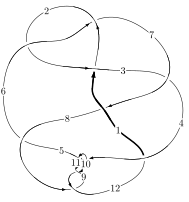
\includegraphics[width=112pt]{../../../GIT/diagram.site/Diagrams/png/1048_12a_0247.png}\\
\ \ \ A knot diagram\footnotemark}&
\allowdisplaybreaks
\textbf{Linearized knot diagam} \\
\cline{2-2}
 &
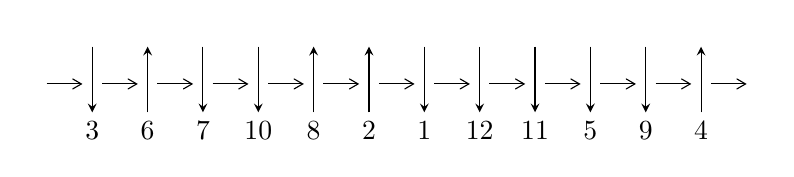
\begin{tikzpicture}[x=20pt, y=17pt]
	% nodes
	\node (C0) at (0, 0) {};
	\node (C1) at (1, 0) {};
	\node (C1U) at (1, +1) {};
	\node (C1D) at (1, -1) {3};

	\node (C2) at (2, 0) {};
	\node (C2U) at (2, +1) {};
	\node (C2D) at (2, -1) {6};

	\node (C3) at (3, 0) {};
	\node (C3U) at (3, +1) {};
	\node (C3D) at (3, -1) {7};

	\node (C4) at (4, 0) {};
	\node (C4U) at (4, +1) {};
	\node (C4D) at (4, -1) {10};

	\node (C5) at (5, 0) {};
	\node (C5U) at (5, +1) {};
	\node (C5D) at (5, -1) {8};

	\node (C6) at (6, 0) {};
	\node (C6U) at (6, +1) {};
	\node (C6D) at (6, -1) {2};

	\node (C7) at (7, 0) {};
	\node (C7U) at (7, +1) {};
	\node (C7D) at (7, -1) {1};

	\node (C8) at (8, 0) {};
	\node (C8U) at (8, +1) {};
	\node (C8D) at (8, -1) {12};

	\node (C9) at (9, 0) {};
	\node (C9U) at (9, +1) {};
	\node (C9D) at (9, -1) {11};

	\node (C10) at (10, 0) {};
	\node (C10U) at (10, +1) {};
	\node (C10D) at (10, -1) {5};

	\node (C11) at (11, 0) {};
	\node (C11U) at (11, +1) {};
	\node (C11D) at (11, -1) {9};

	\node (C12) at (12, 0) {};
	\node (C12U) at (12, +1) {};
	\node (C12D) at (12, -1) {4};
	\node (C13) at (13, 0) {};

	% arrows
	\draw[->,>={angle 60}]
	(C0) edge (C1) (C1) edge (C2) (C2) edge (C3) (C3) edge (C4) (C4) edge (C5) (C5) edge (C6) (C6) edge (C7) (C7) edge (C8) (C8) edge (C9) (C9) edge (C10) (C10) edge (C11) (C11) edge (C12) (C12) edge (C13) ;	\draw[->,>=stealth]
	(C1U) edge (C1D) (C2D) edge (C2U) (C3U) edge (C3D) (C4U) edge (C4D) (C5D) edge (C5U) (C6D) edge (C6U) (C7U) edge (C7D) (C8U) edge (C8D) (C9U) edge (C9D) (C10U) edge (C10D) (C11U) edge (C11D) (C12D) edge (C12U) ;
	\end{tikzpicture} \\
\hhline{~~} \\& 
\textbf{Solving Sequence} \\ \cline{2-2} 
 &
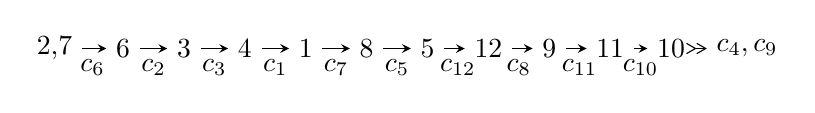
\begin{tikzpicture}[x=22pt, y=7pt]
	% node
	\node (A0) at (-1/8, 0) {2,7};
	\node (A1) at (1, 0) {6};
	\node (A2) at (2, 0) {3};
	\node (A3) at (3, 0) {4};
	\node (A4) at (4, 0) {1};
	\node (A5) at (5, 0) {8};
	\node (A6) at (6, 0) {5};
	\node (A7) at (7, 0) {12};
	\node (A8) at (8, 0) {9};
	\node (A9) at (9, 0) {11};
	\node (A10) at (10, 0) {10};
	\node (C1) at (1/2, -1) {$c_{6}$};
	\node (C2) at (3/2, -1) {$c_{2}$};
	\node (C3) at (5/2, -1) {$c_{3}$};
	\node (C4) at (7/2, -1) {$c_{1}$};
	\node (C5) at (9/2, -1) {$c_{7}$};
	\node (C6) at (11/2, -1) {$c_{5}$};
	\node (C7) at (13/2, -1) {$c_{12}$};
	\node (C8) at (15/2, -1) {$c_{8}$};
	\node (C9) at (17/2, -1) {$c_{11}$};
	\node (C10) at (19/2, -1) {$c_{10}$};
	\node (A11) at (45/4, 0) {$c_{4},c_{9}$};

	% edge
	\draw[->,>=stealth]	
	(A0) edge (A1) (A1) edge (A2) (A2) edge (A3) (A3) edge (A4) (A4) edge (A5) (A5) edge (A6) (A6) edge (A7) (A7) edge (A8) (A8) edge (A9) (A9) edge (A10) ;
	\draw[->>,>={angle 60}]	
	(A10) edge (A11);
\end{tikzpicture} \\ 

\end{tabular} \\

\footnotetext{
The image of knot diagram is generated by the software ``\textbf{Draw programme}" developed by Andrew Bartholomew(\url{http://www.layer8.co.uk/maths/draw/index.htm\#Running-draw}), where we modified some parts for our purpose(\url{https://github.com/CATsTAILs/LinksPainter}).
}\phantom \\ \newline 
\centering \textbf{Ideals for irreducible components\footnotemark of $X_{\text{par}}$} 
 
\begin{align*}
I^u_{1}&=\langle 
u^{81}+u^{80}+\cdots+u-1\rangle \\
\\
\end{align*}
\raggedright * 1 irreducible components of $\dim_{\mathbb{C}}=0$, with total 81 representations.\\
\footnotetext{All coefficients of polynomials are rational numbers. But the coefficients are sometimes approximated in decimal forms when there is not enough margin.}
\newpage
\renewcommand{\arraystretch}{1}
\centering \section*{I. $I^u_{1}= \langle u^{81}+u^{80}+\cdots+u-1 \rangle$}
\flushleft \textbf{(i) Arc colorings}\\
\begin{tabular}{m{7pt} m{180pt} m{7pt} m{180pt} }
\flushright $a_{2}=$&$\begin{pmatrix}0\\u\end{pmatrix}$ \\
\flushright $a_{7}=$&$\begin{pmatrix}1\\0\end{pmatrix}$ \\
\flushright $a_{6}=$&$\begin{pmatrix}1\\u^2\end{pmatrix}$ \\
\flushright $a_{3}=$&$\begin{pmatrix}u\\u^3+u\end{pmatrix}$ \\
\flushright $a_{4}=$&$\begin{pmatrix}- u^3\\u^3+u\end{pmatrix}$ \\
\flushright $a_{1}=$&$\begin{pmatrix}u^3\\u^5+u^3+u\end{pmatrix}$ \\
\flushright $a_{8}=$&$\begin{pmatrix}u^8+u^6+u^4+1\\u^{10}+2 u^8+3 u^6+2 u^4+u^2\end{pmatrix}$ \\
\flushright $a_{5}=$&$\begin{pmatrix}u^{16}+3 u^{14}+5 u^{12}+4 u^{10}+3 u^8+2 u^6+2 u^4+1\\u^{18}+4 u^{16}+9 u^{14}+12 u^{12}+11 u^{10}+6 u^8+2 u^6+u^2\end{pmatrix}$ \\
\flushright $a_{12}=$&$\begin{pmatrix}- u^{11}-2 u^9-2 u^7+u^3\\u^{11}+3 u^9+4 u^7+3 u^5+u^3+u\end{pmatrix}$ \\
\flushright $a_{9}=$&$\begin{pmatrix}- u^{32}-7 u^{30}+\cdots+2 u^4+1\\u^{32}+8 u^{30}+\cdots+4 u^4+2 u^2\end{pmatrix}$ \\
\flushright $a_{11}=$&$\begin{pmatrix}- u^{53}-12 u^{51}+\cdots+2 u^3+u\\u^{53}+13 u^{51}+\cdots+3 u^3+u\end{pmatrix}$ \\
\flushright $a_{10}=$&$\begin{pmatrix}- u^{74}-17 u^{72}+\cdots+u^2+1\\u^{74}+18 u^{72}+\cdots+8 u^4+3 u^2\end{pmatrix}$\\&\end{tabular}
\flushleft \textbf{(ii) Obstruction class $= -1$}\\~\\
\flushleft \textbf{(iii) Cusp Shapes $= -4 u^{80}-4 u^{79}+\cdots-8 u^2-6$}\\~\\
\newpage\renewcommand{\arraystretch}{1}
\flushleft \textbf{(iv) u-Polynomials at the component}\newline \\
\begin{tabular}{m{50pt}|m{274pt}}
Crossings & \hspace{64pt}u-Polynomials at each crossing \\
\hline $$\begin{aligned}c_{1}\end{aligned}$$&$\begin{aligned}
&u^{81}+39 u^{80}+\cdots+u-1
\end{aligned}$\\
\hline $$\begin{aligned}c_{2},c_{6}\end{aligned}$$&$\begin{aligned}
&u^{81}- u^{80}+\cdots+u+1
\end{aligned}$\\
\hline $$\begin{aligned}c_{3}\end{aligned}$$&$\begin{aligned}
&u^{81}+u^{80}+\cdots-277 u+65
\end{aligned}$\\
\hline $$\begin{aligned}c_{4},c_{10}\end{aligned}$$&$\begin{aligned}
&u^{81}- u^{80}+\cdots+u+1
\end{aligned}$\\
\hline $$\begin{aligned}c_{5},c_{12}\end{aligned}$$&$\begin{aligned}
&u^{81}+7 u^{80}+\cdots+2761 u+101
\end{aligned}$\\
\hline $$\begin{aligned}c_{7}\end{aligned}$$&$\begin{aligned}
&u^{81}-5 u^{80}+\cdots-11 u+3
\end{aligned}$\\
\hline $$\begin{aligned}c_{8},c_{9},c_{11}\end{aligned}$$&$\begin{aligned}
&u^{81}+21 u^{80}+\cdots+u+1
\end{aligned}$\\
\hline
\end{tabular}\\~\\
\newpage\renewcommand{\arraystretch}{1}
\flushleft \textbf{(v) Riley Polynomials at the component}\newline \\
\begin{tabular}{m{50pt}|m{274pt}}
Crossings & \hspace{64pt}Riley Polynomials at each crossing \\
\hline $$\begin{aligned}c_{1}\end{aligned}$$&$\begin{aligned}
&y^{81}+7 y^{80}+\cdots+17 y-1
\end{aligned}$\\
\hline $$\begin{aligned}c_{2},c_{6}\end{aligned}$$&$\begin{aligned}
&y^{81}+39 y^{80}+\cdots+y-1
\end{aligned}$\\
\hline $$\begin{aligned}c_{3}\end{aligned}$$&$\begin{aligned}
&y^{81}-25 y^{80}+\cdots-421431 y-4225
\end{aligned}$\\
\hline $$\begin{aligned}c_{4},c_{10}\end{aligned}$$&$\begin{aligned}
&y^{81}-21 y^{80}+\cdots+y-1
\end{aligned}$\\
\hline $$\begin{aligned}c_{5},c_{12}\end{aligned}$$&$\begin{aligned}
&y^{81}+51 y^{80}+\cdots+2274161 y-10201
\end{aligned}$\\
\hline $$\begin{aligned}c_{7}\end{aligned}$$&$\begin{aligned}
&y^{81}+3 y^{80}+\cdots-563 y-9
\end{aligned}$\\
\hline $$\begin{aligned}c_{8},c_{9},c_{11}\end{aligned}$$&$\begin{aligned}
&y^{81}+79 y^{80}+\cdots+9 y-1
\end{aligned}$\\
\hline
\end{tabular}\\~\\
\newpage\flushleft \textbf{(vi) Complex Volumes and Cusp Shapes}
$$\begin{array}{c|c|c}  
\text{Solutions to }I^u_{1}& \I (\text{vol} + \sqrt{-1}CS) & \text{Cusp shape}\\
 \hline 
\begin{aligned}
u &= \phantom{-}0.330756 + 0.928246 I\end{aligned}
 & -1.98935 - 0.55410 I & \phantom{-0.000000 } 0 \\ \hline\begin{aligned}
u &= \phantom{-}0.330756 - 0.928246 I\end{aligned}
 & -1.98935 + 0.55410 I & \phantom{-0.000000 } 0 \\ \hline\begin{aligned}
u &= \phantom{-}0.555231 + 0.887447 I\end{aligned}
 & \phantom{-}4.58988 - 4.17415 I & \phantom{-0.000000 } 0 \\ \hline\begin{aligned}
u &= \phantom{-}0.555231 - 0.887447 I\end{aligned}
 & \phantom{-}4.58988 + 4.17415 I & \phantom{-0.000000 } 0 \\ \hline\begin{aligned}
u &= -0.550578 + 0.902148 I\end{aligned}
 & \phantom{-}4.97491 - 1.96297 I & \phantom{-0.000000 } 0 \\ \hline\begin{aligned}
u &= -0.550578 - 0.902148 I\end{aligned}
 & \phantom{-}4.97491 + 1.96297 I & \phantom{-0.000000 } 0 \\ \hline\begin{aligned}
u &= \phantom{-}0.021905 + 0.940885 I\end{aligned}
 & \phantom{-}4.01374 - 3.02957 I & -4.00000 + 2.75966 I \\ \hline\begin{aligned}
u &= \phantom{-}0.021905 - 0.940885 I\end{aligned}
 & \phantom{-}4.01374 + 3.02957 I & -4.00000 - 2.75966 I \\ \hline\begin{aligned}
u &= \phantom{-}0.631971 + 0.668959 I\end{aligned}
 & \phantom{-}5.23666 + 8.85428 I & \phantom{-}0.25550 - 7.99532 I \\ \hline\begin{aligned}
u &= \phantom{-}0.631971 - 0.668959 I\end{aligned}
 & \phantom{-}5.23666 - 8.85428 I & \phantom{-}0.25550 + 7.99532 I \\ \hline\begin{aligned}
u &= \phantom{-}0.483592 + 0.777442 I\end{aligned}
 & -2.06562 - 0.44729 I & -7.29217 + 1.06967 I \\ \hline\begin{aligned}
u &= \phantom{-}0.483592 - 0.777442 I\end{aligned}
 & -2.06562 + 0.44729 I & -7.29217 - 1.06967 I \\ \hline\begin{aligned}
u &= -0.474582 + 0.979170 I\end{aligned}
 & -0.31365 - 2.38173 I & \phantom{-0.000000 } 0 \\ \hline\begin{aligned}
u &= -0.474582 - 0.979170 I\end{aligned}
 & -0.31365 + 2.38173 I & \phantom{-0.000000 } 0 \\ \hline\begin{aligned}
u &= -0.630050 + 0.657774 I\end{aligned}
 & \phantom{-}5.69407 - 2.69657 I & \phantom{-}1.28923 + 3.02747 I \\ \hline\begin{aligned}
u &= -0.630050 - 0.657774 I\end{aligned}
 & \phantom{-}5.69407 + 2.69657 I & \phantom{-}1.28923 - 3.02747 I \\ \hline\begin{aligned}
u &= \phantom{-}0.580245 + 0.690845 I\end{aligned}
 & -1.70309 + 4.76740 I & -5.47059 - 8.11597 I \\ \hline\begin{aligned}
u &= \phantom{-}0.580245 - 0.690845 I\end{aligned}
 & -1.70309 - 4.76740 I & -5.47059 + 8.11597 I \\ \hline\begin{aligned}
u &= \phantom{-}0.446078 + 1.061030 I\end{aligned}
 & -3.47656 + 3.43189 I & \phantom{-0.000000 } 0 \\ \hline\begin{aligned}
u &= \phantom{-}0.446078 - 1.061030 I\end{aligned}
 & -3.47656 - 3.43189 I & \phantom{-0.000000 } 0 \\ \hline\begin{aligned}
u &= -0.519943 + 1.034750 I\end{aligned}
 & \phantom{-}0.30103 - 3.37806 I & \phantom{-0.000000 } 0 \\ \hline\begin{aligned}
u &= -0.519943 - 1.034750 I\end{aligned}
 & \phantom{-}0.30103 + 3.37806 I & \phantom{-0.000000 } 0 \\ \hline\begin{aligned}
u &= \phantom{-}0.285545 + 1.130800 I\end{aligned}
 & -5.01539 - 0.16721 I & \phantom{-0.000000 } 0 \\ \hline\begin{aligned}
u &= \phantom{-}0.285545 - 1.130800 I\end{aligned}
 & -5.01539 + 0.16721 I & \phantom{-0.000000 } 0 \\ \hline\begin{aligned}
u &= -0.540133 + 0.631709 I\end{aligned}
 & \phantom{-}0.70198 - 1.71974 I & \phantom{-}1.35755 + 3.78809 I \\ \hline\begin{aligned}
u &= -0.540133 - 0.631709 I\end{aligned}
 & \phantom{-}0.70198 + 1.71974 I & \phantom{-}1.35755 - 3.78809 I \\ \hline\begin{aligned}
u &= -0.771211 + 0.309758 I\end{aligned}
 & \phantom{-}3.47094 + 10.85050 I & -1.26204 - 7.02651 I \\ \hline\begin{aligned}
u &= -0.771211 - 0.309758 I\end{aligned}
 & \phantom{-}3.47094 - 10.85050 I & -1.26204 + 7.02651 I \\ \hline\begin{aligned}
u &= \phantom{-}0.249724 + 1.142850 I\end{aligned}
 & -0.48830 - 1.78736 I & \phantom{-0.000000 } 0 \\ \hline\begin{aligned}
u &= \phantom{-}0.249724 - 1.142850 I\end{aligned}
 & -0.48830 + 1.78736 I & \phantom{-0.000000 } 0\\
 \hline 
 \end{array}$$\newpage$$\begin{array}{c|c|c}  
\text{Solutions to }I^u_{1}& \I (\text{vol} + \sqrt{-1}CS) & \text{Cusp shape}\\
 \hline 
\begin{aligned}
u &= -0.683944 + 0.470341 I\end{aligned}
 & \phantom{-}8.62833 - 2.03896 I & \phantom{-}3.69559 + 2.22375 I \\ \hline\begin{aligned}
u &= -0.683944 - 0.470341 I\end{aligned}
 & \phantom{-}8.62833 + 2.03896 I & \phantom{-}3.69559 - 2.22375 I \\ \hline\begin{aligned}
u &= \phantom{-}0.689016 + 0.459096 I\end{aligned}
 & \phantom{-}8.57475 - 4.19689 I & \phantom{-}3.50201 + 3.13868 I \\ \hline\begin{aligned}
u &= \phantom{-}0.689016 - 0.459096 I\end{aligned}
 & \phantom{-}8.57475 + 4.19689 I & \phantom{-}3.50201 - 3.13868 I \\ \hline\begin{aligned}
u &= \phantom{-}0.765943 + 0.314154 I\end{aligned}
 & \phantom{-}4.01700 - 4.68092 I & -0.19311 + 2.19687 I \\ \hline\begin{aligned}
u &= \phantom{-}0.765943 - 0.314154 I\end{aligned}
 & \phantom{-}4.01700 + 4.68092 I & -0.19311 - 2.19687 I \\ \hline\begin{aligned}
u &= -0.250936 + 1.149570 I\end{aligned}
 & -1.05501 + 7.90870 I & \phantom{-0.000000 } 0 \\ \hline\begin{aligned}
u &= -0.250936 - 1.149570 I\end{aligned}
 & -1.05501 - 7.90870 I & \phantom{-0.000000 } 0 \\ \hline\begin{aligned}
u &= -0.275321 + 1.148290 I\end{aligned}
 & -7.91963 + 3.33484 I & \phantom{-0.000000 } 0 \\ \hline\begin{aligned}
u &= -0.275321 - 1.148290 I\end{aligned}
 & -7.91963 - 3.33484 I & \phantom{-0.000000 } 0 \\ \hline\begin{aligned}
u &= \phantom{-}0.333976 + 1.136910 I\end{aligned}
 & -1.43197 + 1.29517 I & \phantom{-0.000000 } 0 \\ \hline\begin{aligned}
u &= \phantom{-}0.333976 - 1.136910 I\end{aligned}
 & -1.43197 - 1.29517 I & \phantom{-0.000000 } 0 \\ \hline\begin{aligned}
u &= -0.301260 + 1.146810 I\end{aligned}
 & -8.21875 - 2.62295 I & \phantom{-0.000000 } 0 \\ \hline\begin{aligned}
u &= -0.301260 - 1.146810 I\end{aligned}
 & -8.21875 + 2.62295 I & \phantom{-0.000000 } 0 \\ \hline\begin{aligned}
u &= -0.755307 + 0.286115 I\end{aligned}
 & -3.56728 + 6.37685 I & -6.68349 - 6.54893 I \\ \hline\begin{aligned}
u &= -0.755307 - 0.286115 I\end{aligned}
 & -3.56728 - 6.37685 I & -6.68349 + 6.54893 I \\ \hline\begin{aligned}
u &= -0.330768 + 1.146950 I\end{aligned}
 & -1.97419 - 7.22380 I & \phantom{-0.000000 } 0 \\ \hline\begin{aligned}
u &= -0.330768 - 1.146950 I\end{aligned}
 & -1.97419 + 7.22380 I & \phantom{-0.000000 } 0 \\ \hline\begin{aligned}
u &= -0.569017 + 1.049970 I\end{aligned}
 & \phantom{-}6.92763 - 2.80448 I & \phantom{-0.000000 } 0 \\ \hline\begin{aligned}
u &= -0.569017 - 1.049970 I\end{aligned}
 & \phantom{-}6.92763 + 2.80448 I & \phantom{-0.000000 } 0 \\ \hline\begin{aligned}
u &= \phantom{-}0.569598 + 1.056390 I\end{aligned}
 & \phantom{-}6.82301 + 9.05454 I & \phantom{-0.000000 } 0 \\ \hline\begin{aligned}
u &= \phantom{-}0.569598 - 1.056390 I\end{aligned}
 & \phantom{-}6.82301 - 9.05454 I & \phantom{-0.000000 } 0 \\ \hline\begin{aligned}
u &= \phantom{-}0.529876 + 1.077230 I\end{aligned}
 & -0.50944 + 7.02202 I & \phantom{-0.000000 } 0 \\ \hline\begin{aligned}
u &= \phantom{-}0.529876 - 1.077230 I\end{aligned}
 & -0.50944 - 7.02202 I & \phantom{-0.000000 } 0 \\ \hline\begin{aligned}
u &= \phantom{-}0.728882 + 0.290469 I\end{aligned}
 & -0.81550 - 3.12081 I & -0.65919 + 2.66104 I \\ \hline\begin{aligned}
u &= \phantom{-}0.728882 - 0.290469 I\end{aligned}
 & -0.81550 + 3.12081 I & -0.65919 - 2.66104 I \\ \hline\begin{aligned}
u &= -0.732942 + 0.254989 I\end{aligned}
 & -4.07021 + 0.53547 I & -8.23201 + 1.09852 I \\ \hline\begin{aligned}
u &= -0.732942 - 0.254989 I\end{aligned}
 & -4.07021 - 0.53547 I & -8.23201 - 1.09852 I \\ \hline\begin{aligned}
u &= \phantom{-}0.512335 + 1.126340 I\end{aligned}
 & -0.22713 + 6.52430 I & \phantom{-0.000000 } 0 \\ \hline\begin{aligned}
u &= \phantom{-}0.512335 - 1.126340 I\end{aligned}
 & -0.22713 - 6.52430 I & \phantom{-0.000000 } 0\\
 \hline 
 \end{array}$$\newpage$$\begin{array}{c|c|c}  
\text{Solutions to }I^u_{1}& \I (\text{vol} + \sqrt{-1}CS) & \text{Cusp shape}\\
 \hline 
\begin{aligned}
u &= -0.578778 + 0.484061 I\end{aligned}
 & \phantom{-}1.91397 - 1.02951 I & \phantom{-}2.98287 + 4.00023 I \\ \hline\begin{aligned}
u &= -0.578778 - 0.484061 I\end{aligned}
 & \phantom{-}1.91397 + 1.02951 I & \phantom{-}2.98287 - 4.00023 I \\ \hline\begin{aligned}
u &= -0.515985 + 1.136090 I\end{aligned}
 & -0.720055 - 0.730088 I & \phantom{-0.000000 } 0 \\ \hline\begin{aligned}
u &= -0.515985 - 1.136090 I\end{aligned}
 & -0.720055 + 0.730088 I & \phantom{-0.000000 } 0 \\ \hline\begin{aligned}
u &= \phantom{-}0.546823 + 1.128660 I\end{aligned}
 & -3.24659 + 7.96298 I & \phantom{-0.000000 } 0 \\ \hline\begin{aligned}
u &= \phantom{-}0.546823 - 1.128660 I\end{aligned}
 & -3.24659 - 7.96298 I & \phantom{-0.000000 } 0 \\ \hline\begin{aligned}
u &= -0.537260 + 1.136870 I\end{aligned}
 & -6.61921 - 5.33206 I & \phantom{-0.000000 } 0 \\ \hline\begin{aligned}
u &= -0.537260 - 1.136870 I\end{aligned}
 & -6.61921 + 5.33206 I & \phantom{-0.000000 } 0 \\ \hline\begin{aligned}
u &= -0.708940 + 0.201872 I\end{aligned}
 & \phantom{-}1.93893 - 3.88483 I & -3.08441 + 2.98468 I \\ \hline\begin{aligned}
u &= -0.708940 - 0.201872 I\end{aligned}
 & \phantom{-}1.93893 + 3.88483 I & -3.08441 - 2.98468 I \\ \hline\begin{aligned}
u &= -0.551751 + 1.137250 I\end{aligned}
 & -6.05282 - 11.29930 I & \phantom{-0.000000 } 0 \\ \hline\begin{aligned}
u &= -0.551751 - 1.137250 I\end{aligned}
 & -6.05282 + 11.29930 I & \phantom{-0.000000 } 0 \\ \hline\begin{aligned}
u &= \phantom{-}0.563166 + 1.133120 I\end{aligned}
 & \phantom{-}1.61264 + 9.68341 I & \phantom{-0.000000 } 0 \\ \hline\begin{aligned}
u &= \phantom{-}0.563166 - 1.133120 I\end{aligned}
 & \phantom{-}1.61264 - 9.68341 I & \phantom{-0.000000 } 0 \\ \hline\begin{aligned}
u &= \phantom{-}0.629075 + 0.379382 I\end{aligned}
 & \phantom{-}1.50547 - 2.46200 I & \phantom{-}0.64686 + 5.57955 I \\ \hline\begin{aligned}
u &= \phantom{-}0.629075 - 0.379382 I\end{aligned}
 & \phantom{-}1.50547 + 2.46200 I & \phantom{-}0.64686 - 5.57955 I \\ \hline\begin{aligned}
u &= -0.563360 + 1.136020 I\end{aligned}
 & \phantom{-}1.0430 - 15.8655 I & \phantom{-0.000000 } 0 \\ \hline\begin{aligned}
u &= -0.563360 - 1.136020 I\end{aligned}
 & \phantom{-}1.0430 + 15.8655 I & \phantom{-0.000000 } 0 \\ \hline\begin{aligned}
u &= \phantom{-}0.684512 + 0.197850 I\end{aligned}
 & \phantom{-}2.38107 - 1.99261 I & -2.22631 + 2.45378 I \\ \hline\begin{aligned}
u &= \phantom{-}0.684512 - 0.197850 I\end{aligned}
 & \phantom{-}2.38107 + 1.99261 I & -2.22631 - 2.45378 I \\ \hline\begin{aligned}
u &= \phantom{-}0.407633\phantom{ +0.000000I}\end{aligned}
 & -1.06455\phantom{ +0.000000I} & -9.20770\phantom{ +0.000000I}\\
 \hline 
 \end{array}$$\newpage
\newpage\renewcommand{\arraystretch}{1}
\centering \section*{ II. u-Polynomials}
\begin{tabular}{m{50pt}|m{274pt}}
Crossings & \hspace{64pt}u-Polynomials at each crossing \\
\hline $$\begin{aligned}c_{1}\end{aligned}$$&$\begin{aligned}
&u^{81}+39 u^{80}+\cdots+u-1
\end{aligned}$\\
\hline $$\begin{aligned}c_{2},c_{6}\end{aligned}$$&$\begin{aligned}
&u^{81}- u^{80}+\cdots+u+1
\end{aligned}$\\
\hline $$\begin{aligned}c_{3}\end{aligned}$$&$\begin{aligned}
&u^{81}+u^{80}+\cdots-277 u+65
\end{aligned}$\\
\hline $$\begin{aligned}c_{4},c_{10}\end{aligned}$$&$\begin{aligned}
&u^{81}- u^{80}+\cdots+u+1
\end{aligned}$\\
\hline $$\begin{aligned}c_{5},c_{12}\end{aligned}$$&$\begin{aligned}
&u^{81}+7 u^{80}+\cdots+2761 u+101
\end{aligned}$\\
\hline $$\begin{aligned}c_{7}\end{aligned}$$&$\begin{aligned}
&u^{81}-5 u^{80}+\cdots-11 u+3
\end{aligned}$\\
\hline $$\begin{aligned}c_{8},c_{9},c_{11}\end{aligned}$$&$\begin{aligned}
&u^{81}+21 u^{80}+\cdots+u+1
\end{aligned}$\\
\hline
\end{tabular}\newpage\renewcommand{\arraystretch}{1}
\centering \section*{ III. Riley Polynomials}
\begin{tabular}{m{50pt}|m{274pt}}
Crossings & \hspace{64pt}Riley Polynomials at each crossing \\
\hline $$\begin{aligned}c_{1}\end{aligned}$$&$\begin{aligned}
&y^{81}+7 y^{80}+\cdots+17 y-1
\end{aligned}$\\
\hline $$\begin{aligned}c_{2},c_{6}\end{aligned}$$&$\begin{aligned}
&y^{81}+39 y^{80}+\cdots+y-1
\end{aligned}$\\
\hline $$\begin{aligned}c_{3}\end{aligned}$$&$\begin{aligned}
&y^{81}-25 y^{80}+\cdots-421431 y-4225
\end{aligned}$\\
\hline $$\begin{aligned}c_{4},c_{10}\end{aligned}$$&$\begin{aligned}
&y^{81}-21 y^{80}+\cdots+y-1
\end{aligned}$\\
\hline $$\begin{aligned}c_{5},c_{12}\end{aligned}$$&$\begin{aligned}
&y^{81}+51 y^{80}+\cdots+2274161 y-10201
\end{aligned}$\\
\hline $$\begin{aligned}c_{7}\end{aligned}$$&$\begin{aligned}
&y^{81}+3 y^{80}+\cdots-563 y-9
\end{aligned}$\\
\hline $$\begin{aligned}c_{8},c_{9},c_{11}\end{aligned}$$&$\begin{aligned}
&y^{81}+79 y^{80}+\cdots+9 y-1
\end{aligned}$\\
\hline
\end{tabular}
\vskip 2pc
\end{document}